\documentclass[a4paper,12pt]{article}

\usepackage{graphicx} % Required for inserting images
\usepackage{amsmath,amssymb,amsfonts}
\usepackage{subcaption}
% -----------------------
% Package Imports
% -----------------------

% Set page margins
\usepackage[a4paper, top=1in, bottom=0.8in, left=1.1in, right=0.8in]{geometry}

% Use Times New Roman font
\usepackage{times}

% Add page numbering
\pagestyle{plain}

% Enable graphics inclusion
\usepackage{graphicx}
\usepackage{float}
% Enable code listings
\usepackage{listings}
\usepackage{xcolor} % For customizing code colors
\setlength{\parindent}{0pt}

\begin{document}

\section{Experiment No. 2}

\section{Experiment Title }
Design and Analyze CMOS Inverter and Tristate Inverter ensuring proper DRC using MICROWIND 3.0
\section{Objective}
The main objectives of this report are:

\begin{itemize}
	\item To design and simulate a CMOS inverter using MICROWIND 3.0.
	\item To ensure proper compliance with Design Rule Check (DRC) requirements during the design process.
	\item To design and simulate a tri-state inverter using MICROWIND 3.0
	\item To analyze the functionality and switching characteristics of both CMOS and tri-state inverters.
\end{itemize}
\section{Theory}

\subsection{CMOS Inverter}
A CMOS inverter, also known as a complementary metal-oxide-semiconductor inverter, is the most basic building block in digital electronics. It consists of a PMOS (p-type MOSFET) and an NMOS (n-type MOSFET) transistor connected in a complementary manner. The CMOS inverter has two input states: logic 0 (low) and logic 1 (high). The output switches between the supply voltage (logic 1) and ground (logic 0), depending on the input.
\begin{figure}[H]
	\centering
	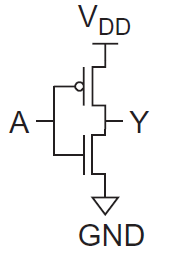
\includegraphics[width=0.2\linewidth]{images/c/ci1.2}
	\caption{CMOS Inverter}
	\label{fig:ci1}
\end{figure}

\textbf{Truth Table for CMOS Inverter:}

\begin{table}[H]
	\centering
	\begin{tabular}{|c|c|}
		\hline
		\textbf{Input (A)} & \textbf{Output (Y)} \\
		\hline
		0 & 1 \\
		1 & 0 \\
		\hline
	\end{tabular}
	\caption{Truth table of CMOS inverter}
\end{table}

The PMOS transistor is ON when the input is low (logic 0), connecting the output to the supply voltage (V\textsubscript{DD}), producing a logic high output. The NMOS transistor is OFF in this state, preventing current from flowing to the ground. Conversely, when the input is high (logic 1), the NMOS transistor is ON, connecting the output to ground (logic 0), while the PMOS transistor is OFF. This complementary action ensures low power dissipation, as current flows only during switching events.

\subsection{Tri-state Inverter}
A tri-state inverter extends the functionality of a CMOS inverter by adding an enable signal, which controls the output state. In addition to logic 0 and 1, the tri-state inverter can have a high-impedance state (Z), which effectively disconnects the output from the circuit. This is useful in bus systems where multiple devices share the same communication line.
\begin{figure}[H]
	\centering
	\begin{subfigure}[t]{0.30\textwidth}
		\centering
		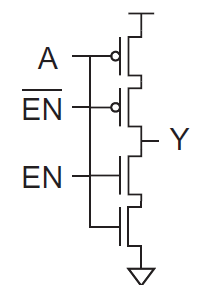
\includegraphics[width=.89\linewidth]{images/t/ti1.2}
		\caption{Tristate Inverter}
	\end{subfigure}
	\hfill
	\begin{subfigure}[t]{0.3\textwidth}
		\centering
		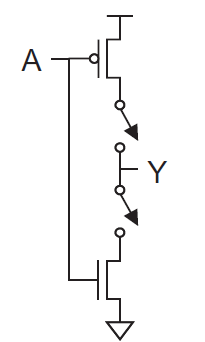
\includegraphics[width=.75\linewidth]{images/t/ti2}
		\caption{EN=0 , Y='Z'}
	\end{subfigure}
	\hfill
	\begin{subfigure}[t]{0.3\textwidth}
		\centering
		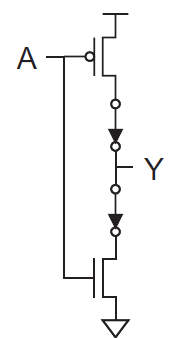
\includegraphics[width=.75\linewidth]{images/t/ti3}
		\caption{EN=1 , Y=$\bar{A}$}
	\end{subfigure}
	\caption{Tristate Inverter }
\end{figure}
\textbf{Truth Table for Tri-state Inverter:}

\begin{table}[h!]
	\centering
	\begin{tabular}{|c|c|c|}
		\hline
		\textbf{Input (A)} & \textbf{Enable (EN)} & \textbf{Output (Y)} \\
		\hline
		0 & 1 & 1 \\
		1 & 1 & 0 \\
		X & 0 & Z \\
		\hline
	\end{tabular}
	\caption{Truth table of tri-state inverter}
\end{table}

When the enable signal (E) is active (logic 1), the inverter behaves like a normal CMOS inverter, producing an inverted output. When the enable signal is low (logic 0), the output enters a high-impedance (Z) state, effectively disconnecting it from the circuit.
\newpage
\subsection{Working Process of Designing a CMOS Inverter using MICROWIND 3.0}
Designing a CMOS inverter in MICROWIND 3.0 involves the following steps:

\begin{enumerate}
	\item \textbf{Create a New Layout:} Open MICROWIND 3.0 and create a new project. The tool provides a blank canvas for designing the layout at the transistor level.
	\item \textbf{Place PMOS and NMOS Transistors:} Using MOS Generator, place a PMOS transistor in the upper part of the layout and an NMOS transistor in the lower part. The transistors are connected at the output node.
	\item \textbf{Connect Power and Ground:} Connect the source of the PMOS to the power supply (V\textsubscript{DD}) and the source of the NMOS to the ground.
	\item \textbf{Define Input and Output:} The input is connected to the gates of both the PMOS and NMOS transistors, while the output is taken from the common drain terminal.
	\item \textbf{Run DRC:} After completing the layout, run the DRC tool to ensure that the design follows all the required fabrication rules.
	\item \textbf{Simulate the Inverter:} Perform a transient simulation to observe the input-output behavior and verify the inverter operation.
\end{enumerate}

\subsection{Working Process of Designing a Tri-state Inverter using MICROWIND 3.0}
Designing a tri-state inverter follows a similar process but with an additional enable signal. The steps are as follows:

\begin{enumerate}
	\item \textbf{Create a New Layout:} Start a new project in MICROWIND 3.0.
	\item \textbf{Place Transistors:} Place PMOS and NMOS transistors as in the CMOS inverter design. Additionally, include a control transistor that manages the enable signal.
	\item \textbf{Connect Enable Signal:} The enable signal controls whether the output is active or in a high-impedance state by controlling DC power supply.
	\item \textbf{Connect Input and Output:} Connect the input to the gates of the PMOS and NMOS transistors. The output is taken from the drains.
	\item \textbf{Run DRC:} Check the layout using the DRC tool to ensure that no design rules are violated.
	\item \textbf{Simulate the Tri-state Inverter:} Simulate the inverter to check how the circuit behaves with the enable signal in both active and inactive states.
\end{enumerate}



\newpage
\section{Schematic Layout }
\begin{figure}[H]
	\centering

\begin{subfigure}[t]{0.49\textwidth}
	\centering

		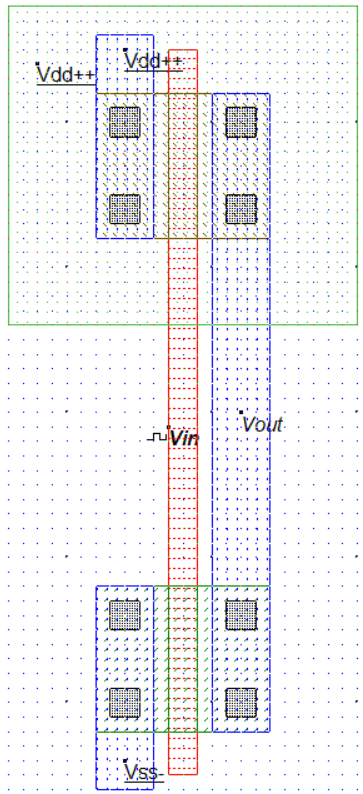
\includegraphics[width=.9\linewidth, height=.7\textheight]{images/c/ci1}

	\caption{CMOS Inverter}

	\label{fig:ci1}
\end{subfigure}
\hfill
\begin{subfigure}[t]{0.49\textwidth}
	\centering
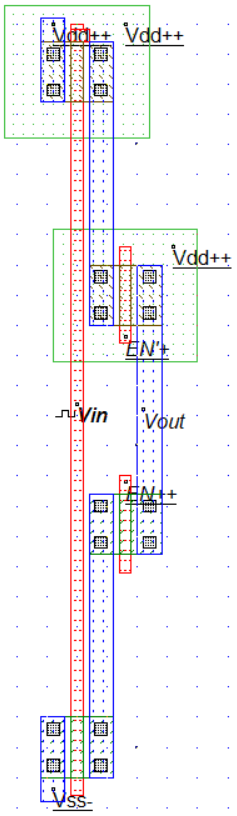
\includegraphics[width=.8\linewidth]{images/t/ti1}
\caption{Tristate Inverter}
\label{fig:ci1}
\end{subfigure}
\caption{Design layout of CMOS Inverter and Tristate Inverter}
\end{figure}

\newpage
\section{Specification}
\begin{enumerate}
\item \textbf{CMOS Inverter}
\begin{figure}[H]
	\centering
	\begin{subfigure}[t]{0.32\textwidth}
		\centering
		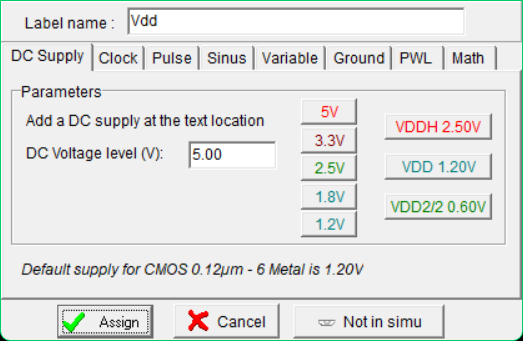
\includegraphics[width=1\linewidth]{images/c/vdd1}
		\caption{Vdd}
	\end{subfigure}
	\hfill
	\begin{subfigure}[t]{0.32\textwidth}
		\centering
		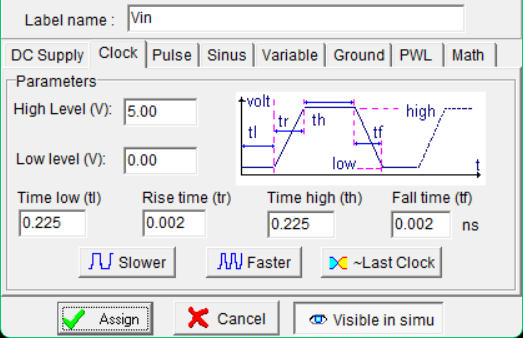
\includegraphics[width=1\linewidth]{images/c/vin}
		\caption{Vin}
	\end{subfigure}
	\hfill
	\begin{subfigure}[t]{0.32\textwidth}
		\centering
		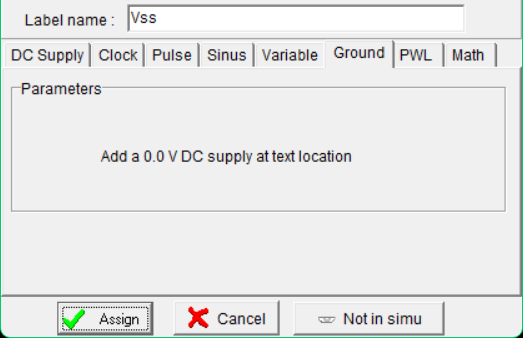
\includegraphics[width=1\linewidth]{images/c/vss}
		\caption{Vss}
	\end{subfigure}
		\caption{Specifications of CMOS Inverter }
\end{figure}

\item \textbf{Tristate Inverter}
\begin{figure}[H]
	\centering
	\begin{subfigure}[t]{0.33\textwidth}
		\centering
		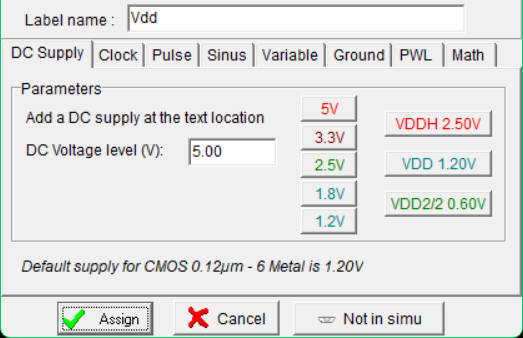
\includegraphics[width=1\linewidth]{images/t/vdd}
		\caption{Vdd}
	\end{subfigure}
	\hfill
	\begin{subfigure}[t]{0.32\textwidth}
		\centering
		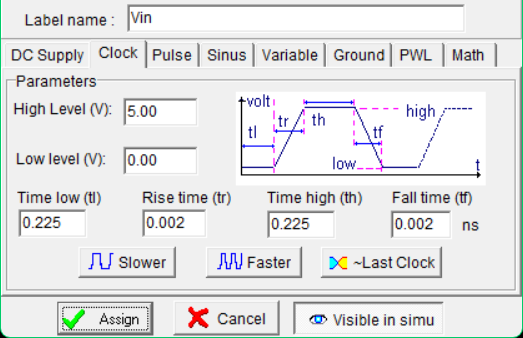
\includegraphics[width=1\linewidth]{images/t/vin}
		\caption{Vin}
	\end{subfigure}
	\hfill
	\begin{subfigure}[t]{0.32\textwidth}
		\centering
		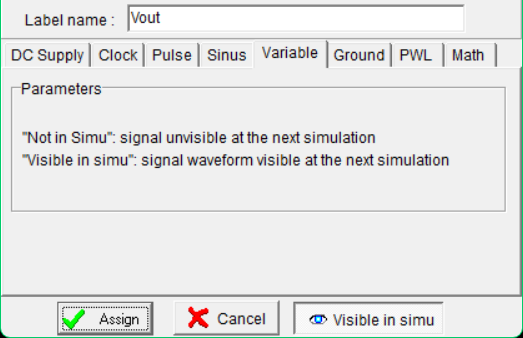
\includegraphics[width=1\linewidth]{images/t/vout}
		\caption{Vout}
	\end{subfigure}
	

	\begin{subfigure}[t]{0.32\textwidth}
		\centering
		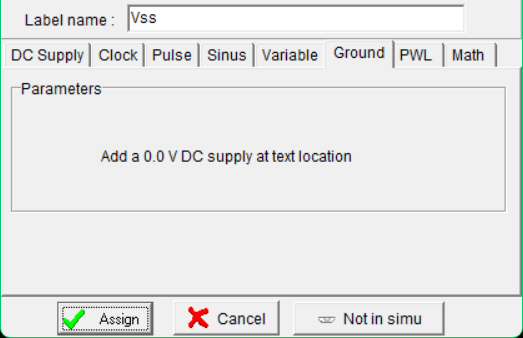
\includegraphics[width=1\linewidth]{images/t/vss}
		\caption{Vss}
	\end{subfigure}
	\hfill
	\begin{subfigure}[t]{0.32\textwidth}
		\centering
		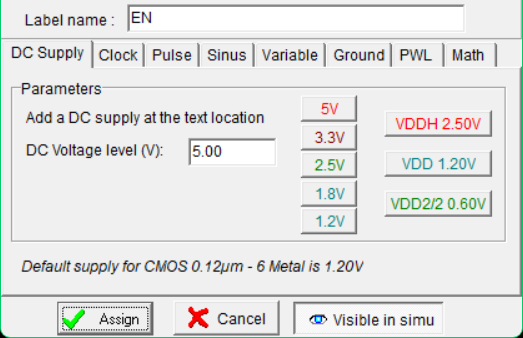
\includegraphics[width=1\linewidth]{images/t/en}
		\caption{EN}
	\end{subfigure}
	\hfill
	\begin{subfigure}[t]{0.32\textwidth}
		\centering
		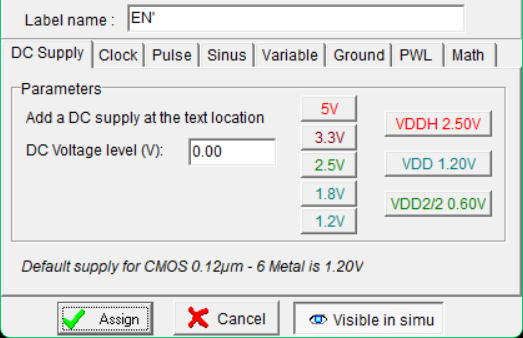
\includegraphics[width=1\linewidth]{images/t/en'}
		\caption{EN'}
	\end{subfigure}
	\caption{Specifications of Tristate Inverter}
\end{figure}

\end{enumerate}



\newpage
\section{Output Waveshape }
	\begin{figure}[H]
	\centering
	\begin{subfigure}[t]{1\textwidth}
		\centering
		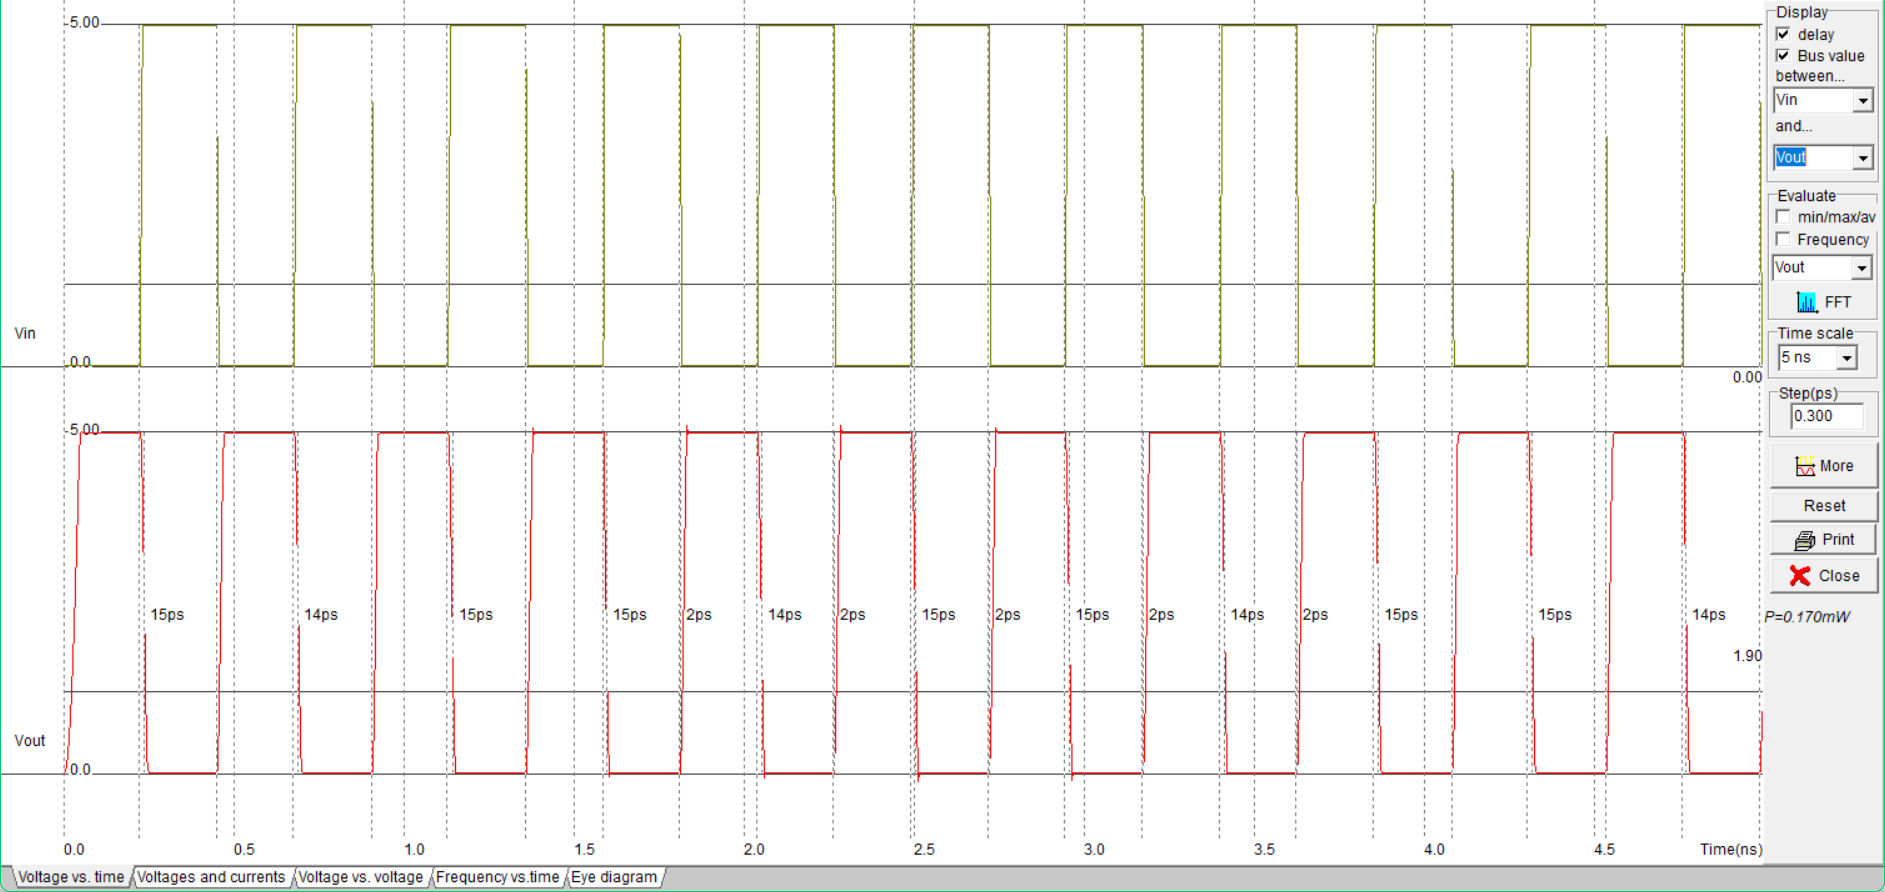
\includegraphics[width=1\textwidth, height=0.27\textheight]{images/c/cisim1}
		\caption{CMOS Inverter}
		\label{fig:1}
	\end{subfigure}
%	\\[1cm]
	\begin{subfigure}[t]{1\textwidth}
		\centering
			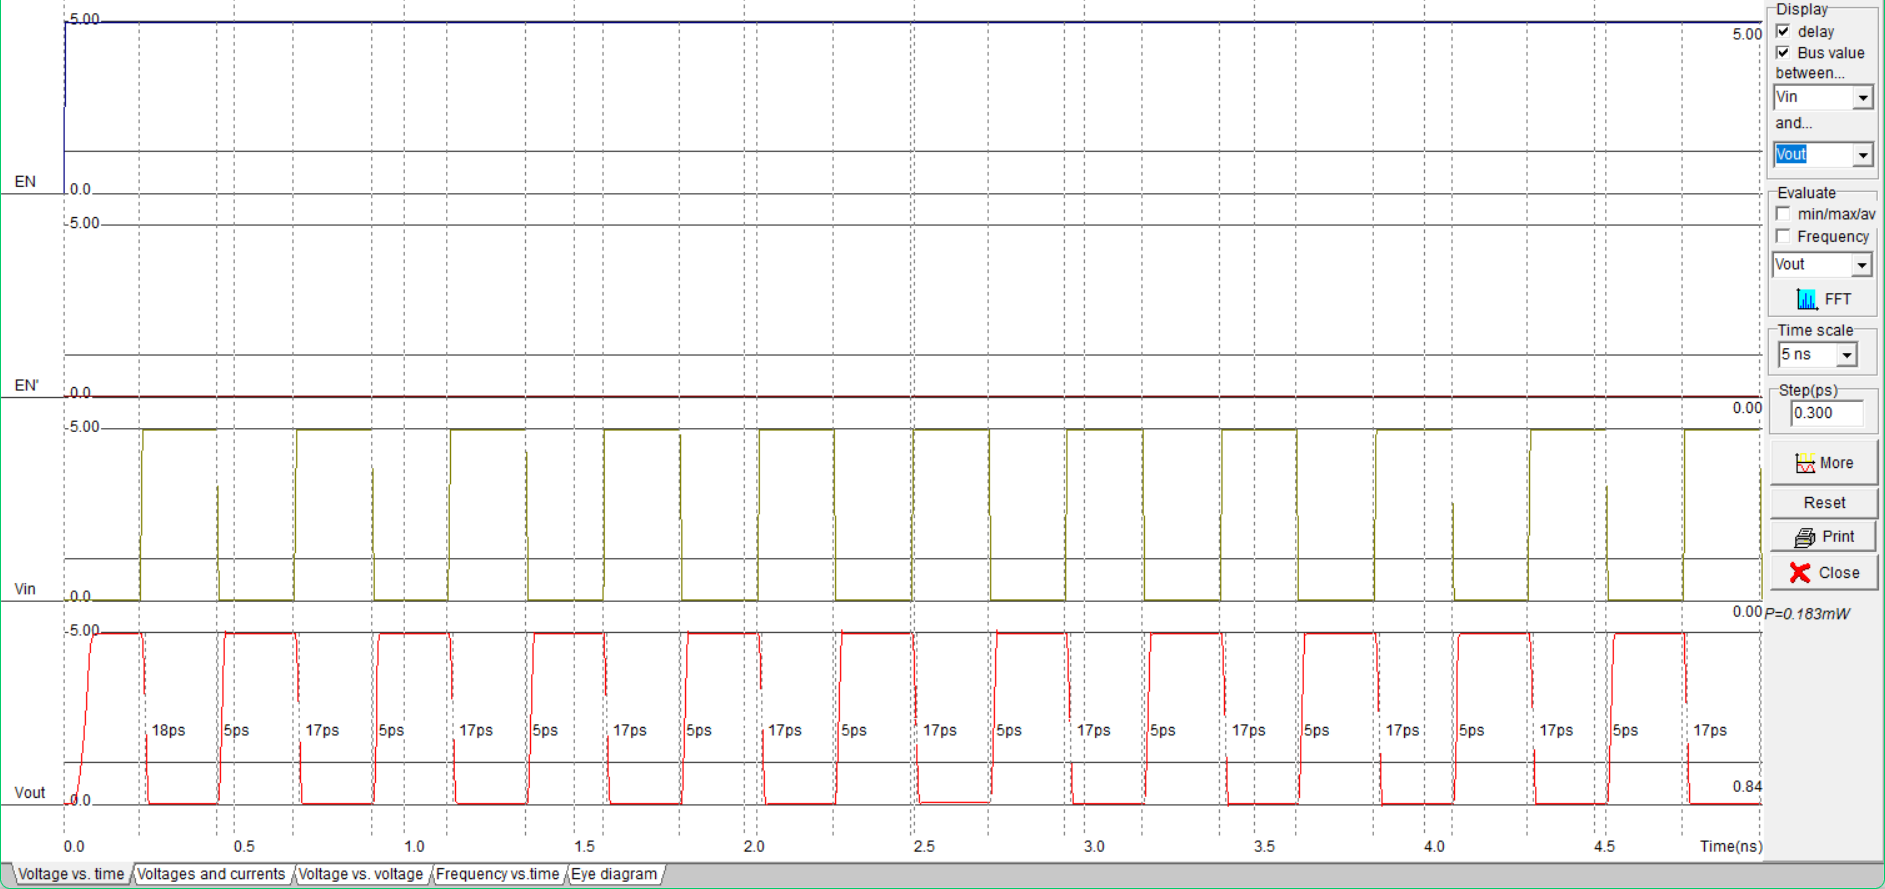
\includegraphics[width=1\linewidth, height=0.29\textheight]{images/t/tisim1}
		\caption{Tristate Inverter when EN=5.00V \& EN'=0.00V}
		\label{fig:2}
	\end{subfigure}
	
		\begin{subfigure}[t]{1\textwidth}
		\centering
		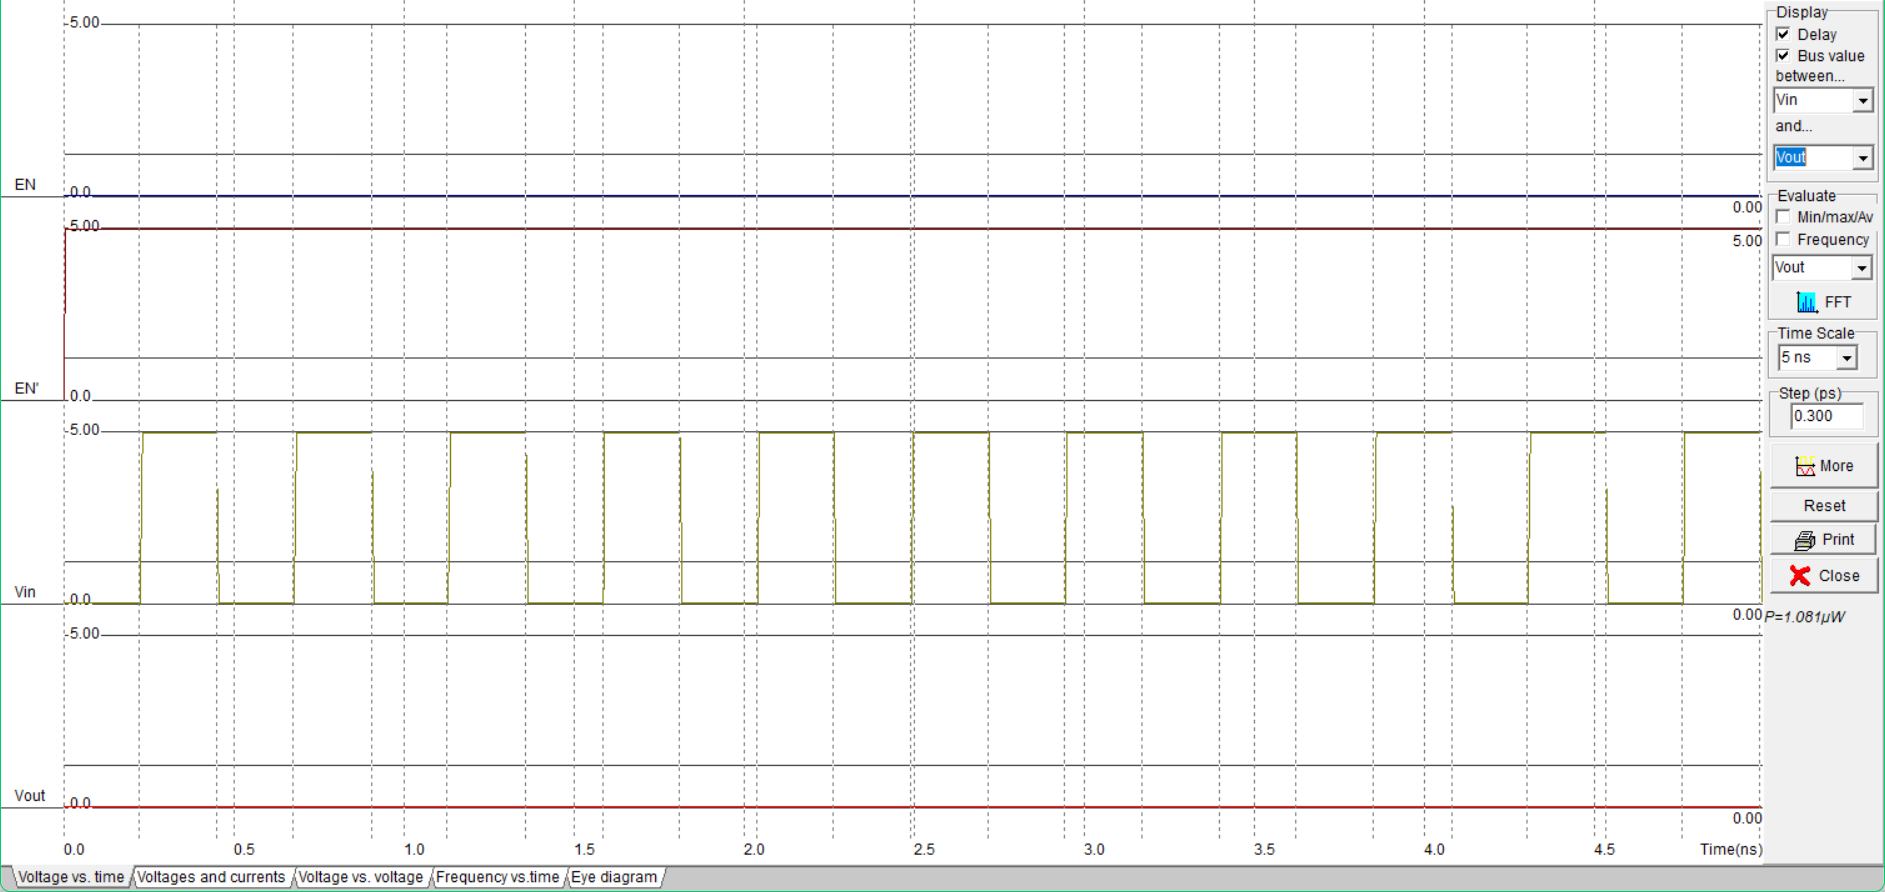
\includegraphics[width=1\linewidth, height=0.29\textheight]{images/t/tisim2}
		\caption{Tristate Inverter when EN=0.00V \& EN'= 5.00V}
		\label{fig:2}
	\end{subfigure}
	\caption{Output Waveshape of Fabricated CMOS Inverter and Tristate Inverter}
\end{figure}

\newpage
\section{Discussion }


In this experiment, the design and analysis of CMOS and tri-state inverters were carried out using MICROWIND 3.0, with particular emphasis on ensuring proper Design Rule Check (DRC) compliance. The CMOS inverter was designed by placing a PMOS and NMOS transistor in a complementary configuration. The input signal $(Vin)$was connected to the gates of both transistors, while the output$(Vout)$ was obtained from the common drain. It was observed during the simulation that the inverter properly switched between logic states, confirming the correct operation of the device.\\
For the tri-state inverter, instead of using an additional transistor, enable signals EN and EN' were manually created. These signals controlled the output state, with EN connected to 5V and EN' to 0V, and vice versa. The inverter successfully transitioned between active and high-impedance states during the simulation, validating the manual control of the enable signals.\\
Overall, the designs were successfully simulated, with both inverters meeting the required operational characteristics. The low power dissipation of the CMOS inverter and the correct functionality of the tri-state inverter in managing output states were observed, confirming the designs' effectiveness.


\end{document}